\documentclass[prl,twocolumn]{revtex4-1}
\usepackage{graphicx}
\usepackage{amsmath}
\usepackage{hyperref}
\usepackage{booktabs}
\usepackage{xcolor}

\usepackage{siunitx}

\setlength{\tabcolsep}{10pt}

\newenvironment{sistema}%
  {\left\lbrace\begin{array}{@{}l@{}}}%
  {\end{array}\right.}



\begin{document}
\title{Gelation as a condensation frustrated by hydrodynamics and mechanical tension}
\author{Hideyo Tsurusawa}
\author{Mathieu Leocmach}
\author{Hajime Tanaka}
\maketitle

\section{Abstract}
Condensations are universal phenomenon in aggregating molecules.
The molecules form droplets and crystals as equilibrium states and gels as non-equilibrium states.
Gels, space-spanning networks with their dynamics arrested, have elasticity and are observed in many systems, including polymers and proteins.
Since open network structures of gels are energetically disfavoured, the mechanism to self-assemble networks has received considerable attentions.
Previously, simulation works have aimed reproducing the process of network formation.
The results of Brownian dynamics simulations, which assume thermal fluctuations and short-range attractions between molecules, have shown formation of droplets in a moderate strength of attractions.
In contrast, the simulations that also consider hydrodynamic interactions can reconstitute gelation in a moderate strength of attractions, suggesting key roles of hydrodynamic interactions in network formation.
However, little is known experimentally about the gelation process because the previous method limits access to the process itself.
Here, we observe the entire process of gelation in a single particle level by a new experimental method and demonstrate that gelation is not a simple condensation but frustrated by hydrodynamic interactions and mechanical tension.

\section{Introduction} % Introduction, from wide attentions to specific subjects
% General attentions
Gels are space-spanning networks with their dynamics arrested, which cause elasticity and are widely used in our daily life such as food and filter.
In a scientific viewpoint, gels have received wide attentions because gels are non-equilibrium non-ergodic states.
% Focusing on 'colloidal gels'
Among various model systems, colloidal gels have been intensively studied since colloids have a great advantage of a single particle resolution.
% AO attraction
Addition of polymer can induce inter-particle attractions, which gelation requires.
As the polymer concentration increases, the attraction strength increases.
% Summary
Therefore, colloid – polymer mixtures have both a single particle resolution and tunabilities of inter-particle attractions.



% Explaining previous works on colloidal gelation
% Phase diagram
Previous works have focused on the phase diagram of colloidal gels and revealed that the gelation boundary is close to the boundary of spinodal decomposition.
% Importance of formation process
But open network structures of gels are energetically disfavored and the mechanism to self-assemble network structures, competing with condensation, is still controversial.
% Formation process / simulation works
Numerical simulation works have studied the formation process of gels.
Tanaka and Araki have compared simulations with and without hydrodynamic interactions and suggested that hydrodynamic interactions may play key roles in network formation.
% Define our problem
However, there are little experimental evidences of the gelation ‘ process ’ in colloidal suspensions because the previous method severely limits access to the formation process.
% Our solution
Here, we observe the ‘ entire process ’ of gelation in a single particle level by a new experimental method and reveal that gelation is not a simple condensation but frustrated by hydrodynamic interactions and mechanical tensions.



\section{New method} % Method of salt reservoir cell
% Principle
Colloidal gels require three components in a solvent: colloid, polymer, and salt.
Polymers are added to induce inter-particle attractions, whereas the salt is needed to screen surface charges of colloids.
If the system contains no salt, colloids can hardly aggregate because of the strong electrostatic repulsions.
% Implementation
Figure~\ref{fig:methods}a shows the schematic diagram of our cell system.
Initially, colloid – polymer mixture without salt are incubated into the observation cell.
Next, salt is added into the reservoir cell and observation is started.
After the salt passes through the filter, the surface charges of colloids are screened and colloids start gelation.
% Validity
Figure~\ref{fig:methods}c-h shows an example of gelation.
At t = 0 min, almost all colloids are dispersed by electrostatic repulsions.
At t = 5 min, the salt diffuses into the observation cell and initiates gelation.
At t = 30 min, the system percolates.
By the new method, we can access the entire process of gelation in a single particle level.





\section{Cluster aggregation} % Subject I: Cluster formation
% Topic sentence
Figure~\ref{fig:methods}a shows the phase diagram of all samples.
First of all, we focus on cluster formation since clusters constitute " building blocks " of gels.
% Results of birth
Figure~\ref{fig:fluid_dilute} a shows the compaction dynamics of the clusters with three colloids in the early stage.
The results show that the clusters can hardly accomplish compaction within one Brownian motion time and clusters with four and five colloids show very similar tendency (Supplement).
% Explanation 1) Local energy minimization.
If one assumes that each colloid can move independently by Brownian motion and static short-range attractions are induced between colloids, the clusters with three colloids should reach the compact states within one Brownian motion time.
This explanation contradicts to our results.
% Addressing our question
In other words, some interactions stabilize linear structures, competing with the principle of energy minimization.
% Explanation 2) Electrostatic repulsion.
Although the effect of electrostatic repulsions has been studied, our results are observed after salt screens surface charges and electrostatic repulsions can be negligible in our system.
% Explanation 3) Hydrodynamic interactions.
Thus, the only possible explanation is the effect of hydrodynamic interactions.
Hydrodynamic interactions originate from the incompressivility of the solvent, whose effect between colloids have been demonstrated by both numerical simulations and the experiments of optical tweezers.
For compaction, clusters must squeeze the solvent inside the cluster to the outside.
% Conclusion.
Our results suggest that squeezing process can be the bottleneck of compaction and hydrodynamic interactions enhance linear structures in clusters.



% Results of growth
% topic sentence
To investigate whether clusters can reach compact states in their growing stage, fractal dimension of each time is analysed in Figure~\ref{fig:fluid_dilute}b.
% General explanation about fractal dimension.
In general, compact clusters have df around three, whereas chain-like clusters have df around one.
%Our results of fractal dimensions
Our results show that df increases from 1 in the early stage to 2 in the late stage but df is much lower than three.
% Explanation 1) DLCA
Previously diffusion limited cluster aggregation model has been proposed to explain uncompact structures of clusters, assuming sticky attractions.
But DLCA model predicts that df is always fixed around 1.85, which contradicts to our results.
% Addressing our question
Therefore, other mechanism should decrease df close to 1 from condensation equilibrium.
% Explanation 2) Hydrodynamic interactions
As discussed in the early stage of cluster formation, hydrodynamic interactions can frustrate condensation of clusters.
If clusters form chain-like structures, clusters can both avoid squeezing process and decrease resistance from external flow.
Therefore, structures of df = 1 are hydrodynamically favored though energetically disfavored.
% Conclusion
Our results suggest that hydrodynamic interactions dominate the system in the early stage.
As the cluster aggregation proceeds, each colloid can access to a more compact state, squeezing out the solvent in the cluster, and df gradually increases.




\section{Dilute gels} % Subject II: Dilute gels
% Topic sentence
Next, we focus on the mechanism of gelation in a dilute system.
% Our results
Figure~\ref{fig:general}c-h shows the process of gelation of phi = 7\%.
Clusters grow by connecting with each other and the radius of gyration of the biggest cluster finally becomes comparable to the system size as shown in Figure~\ref{fig:fluid_dilute}c. 
Figure~\ref{fig:fluid_dilute}b shows that fractal dimension of clusters increase from 1 in the early stage to 2 in the late stage as similar with the case of cluster aggregation.
% Addressing our question
One can address a natural question about dilute gels: Why can the system percolate with phi of only 7\%?
% Introduction to effective phi
Number density of colloids has little importance since fractal dimension of the system is much lower than three and it changes during the gelation process.
% Procedure to calculate the effective volume
To calculate the ‘ effective ’ volume fraction of colloid, we replace each cluster with the effective sphere whose radius is equal to the radius gyration of the cluster.
% Results of effective phi
As shown in Figure~\ref{fig:fluid_dilute}, the effective volume fraction increases from 7\% in the early stage to 60\% in the late stage.
% Discuss the mechanism of percolation in a dilute gel
Our results clearly reveal that the system cannot avoid percolation because the effective volume fraction is too high.
The reason for the 10 times increase of the effective phi is that df is much lower than three.
The low df originates from hydrodynamic interactions.
% Conclusion
Therefore, percolation in a dilute system is a consequence of condensation frustrated by hydrodynamic interactions.





\section{Dense gels} % Subject III: Dense gels
% Topic sentence
Gelation in a dense system, on the other hand, behaves different patterns than in a dilute system.
% Results of the entire process of dense gelation
As shown in Figure~\ref{fig:dense}a, the system accomplishes percolation in a few minutes, whereas coarsening process proceeds for several hours.
% Focusing on percolation mechanism
% Results of percolation
When the system percolates at t = 5 min, the averaged number of nearest neighbours is only three and the averaged bond-bond angle is 105 deg.
Thus, the network right after percolated has chain-like structures instead of condensed domains.
% Discussions of percolation
As shown in Figure~\ref{fig:fluid_dilute}a, the aggregated clusters in the early stage have linear structures by the effect of hydrodynamic interactions.
In a dense system, linear clusters are generated simultaneously in a high density.
The clusters connect with each other before they can reach compact states and form chain-like networks within a few Tb.
% Conclusion
Therefore, percolation in a dense system is a consequence of condensation frustrated by hydrodynamic interactions.

% Focusing on coarsening mechanism
The coarsening proceeds for a long term.
% General discussion
So, each colloid can access an energetically favoured structure by thermal fluctuations.
As condensation proceeds, each colloid is captured in a ‘ cage ’ of nearest neighbours and finally arrested in a deep energy potential.
This model is consistent with the previous suggestions based on the glass transition.
% Introduction for elementary process of coarsening
But the elementary process of coarsening has been unknown.
In the early stage at t = 5 min, more than 99\% of all colloids connect with a single network.
When one colloid moves to form a compact domain, the network interconnected with the colloid should cooperatively move.
Therefore, coarsening process is frustrated by mechanical tensions and the mechanism to overcome the frustration for further condensation has great importance in basic research.
% Results of NW cutting
Figure~\ref{fig:dense}b-d shows an elementary process of coarsening, in which networks coarsens by seizing a part of the network.
The single strand is strained between two strong chains.
After stretched straight, the strand is seized and the fragments are integrated into strong chains.
% Conclusion of elementary process of NW coarsening
Therefore, the system can selectively seize weak chains of the network by inducing mechanical tensions and condensation proceeds until the local structures of the network are strong enough.




\section{Conclusion} % Conclusion of this study
% Topic sentence
In this study, we analyse the entire process of colloidal gelation in a single particle level.
% Universality of colloidal gelation
To show the universality of colloidal gelation, Figure~\ref{fig:general} summarizes the processes of all our data of gel samples.
In a dilute system, local condensation proceeds simultaneously as percolation.
In contrast, dense systems accomplish percolation in the early stage, whereas local condensation proceeds until the late stage.
% Conclusion of colloidal gelation
In both cases of gelation, percolation is a consequence of condensation frustrated by hydrodynamic interactions, whereas the coarsening process is frustrated by mechanical tensions.
%General impacts
Generally, colloidal suspensions are model cases of the binary mixtures that consist of small and big components.
Our study shed a new light on not only colloidal gelation but also dynamically asymmetric mixtures, which include polymer solutions and protein solutions. 




\section{Materials} % Materials and others
% Materials
We use poly-methyl-methacrylate colloids with its radius of \unit{1.4}{\micro\metre} with steric stabilizer of methacryloxypropyl terminated polydimethylsiloxane ( Glest ) dispersed in a mixture of cis-decalin (Tokyo Kasei) and bromocyclohexane ( Sigma-Aldrich ) that matches both optical index and density of the colloids.
The non-adsorbing polymer is \unit{8.4}{\mega\dalton} polystyrene ( TOSOH ) whose radius of gyration in theta solvent is estimated to \unit{110}{\nano\metre}. 
Here the solvent may be regarded as ``good'' and $25\%–40\%$ swelling of the polymer coils is expected~\cite{Royall2007}. We estimate the range of the interaction potential to \unit{148}{\nano\metre} by direct measurements~\cite{Royall2007}, which corresponds to $35\%$ swelling leading to a polymer-colloid size ratio $q=0.05$.

In the absence of salt, the Debye length is expected to reach \unit{???}{\nano\metre}.
Screening by tetrabutylammonium bromide (Fluka) at saturated concentration  brings down the Debye length to about \unit{13}{\nano\metre}.

% Salt-reservoir system
%% Design of the cell
The observation cell has a thickness of approximately \unit{200}{\micro\metre}, whose volume is approximately 1/400 of the volume of the reservoir.
The filter is ??? with pore size of \unit{100}{\nano\metre}.
%% Experimental procedure
Initially, mixture of colloid and polymer without salt is incubated into the observation cell and solvent without salt is incubated into the reservoir.
The reservoir is half-opened and we exchange the solvent into the solvent with salt.
Then, scan starts within \unit{30}{\second}.
%% Results
We estimate that the diffusion time of salt is the order of \unit{10}{\second} as ???.
In our experiments, the colloids in the top area of scan volume start aggregation \unit{1}{\min} after the colloids in the bottom area started aggregation.
Therefore, salt diffuses into the observation cell within only several $\tau_B$.

% Microscope system
Colloids are fluorescently labeled with rhodamines  and observed three-dimensionally by a laser-scanning confocal microscope (Leica SP-5) equipped with excitation laser with its wavelength of \unit{532}{\nano\metre}.
The scan volume is \unit{82 \times 82 \times 85}{\micro\metre} or larger.
We carefully set the scanning time in order to track more than \unit{98}\% of colloids between two continuous time steps.

% Analysis
%% Calculate center positions of colloids
For single-particle analysis, the center position of each colloid is calculated from the three-dimensional images by the algorithm shown in ???.
Trajectory of each colloid is calculated by the algorithm of ???.
%% Identify 'bond'
Colloid A and B are defined as bonded if the distance between the two colloids is smaller than a threshold.
We define the threshold as the first minimum of $g(r)$ of a typical gel samples and apply it for all samples.
%% Identify 'cluster'
By linking all bonds, all clusters are identified and radius gyration and size of each cluster are calculated.
Fractal dimension is calculated by fitting size $r_g\propto N^{d_f}$.
%% Track clusters
To analyse compaction dynamics of clusters with three colloids, we search trajectory of each colloid such that the size of the cluster that contains the colloid is equal to three for continuous time steps.
%% Colouring the picture of cutting NW
???.


\clearpage
\begin{figure}
	\begin{center}
	\includegraphics{generate-figure0.pdf}
	\end{center}
	\caption{\textbf{Observing gelation.} \textbf{a} Sketch of our experimental setup. The observation cell contains initially colloids, polymer and no salt. \textbf{b} Phase diagram of our system (the line is a guide for the eye). \textbf{c-h} Early stage of gelation observed experimentally (state point is circled in \textbf{b}). Pictures are computer reconstruction of the experimental coordinates coloured by the number of particles in clusters.}
	\label{fig:methods}
\end{figure}

\clearpage
\begin{figure}
	\begin{center}
	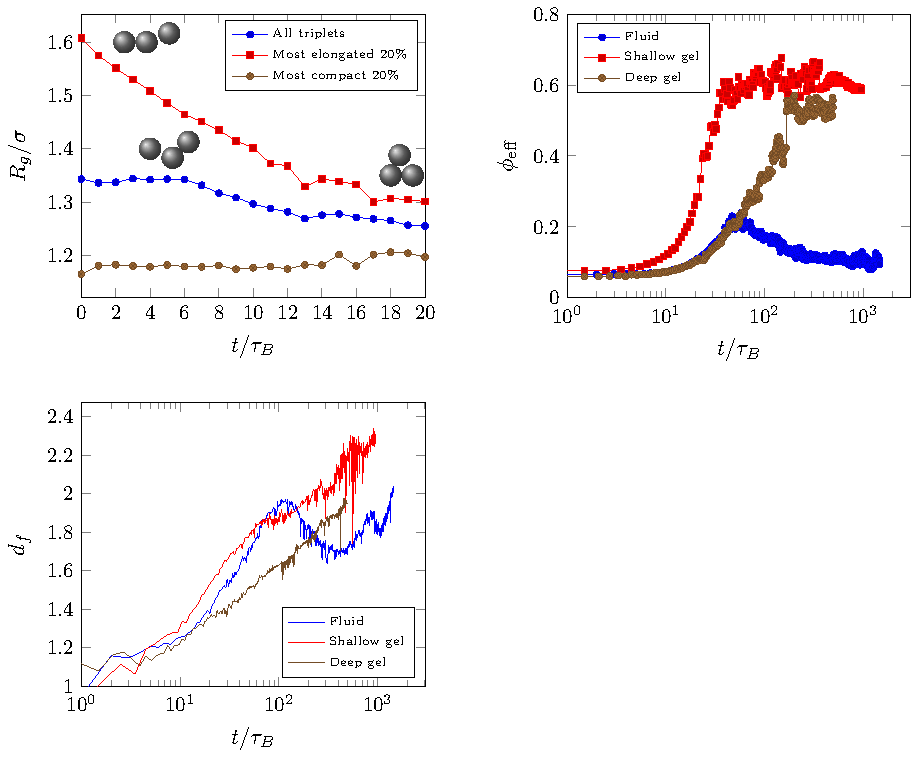
\includegraphics{generate-figure1.pdf}
	\end{center}
	\caption{\textbf{Fluid and dilute gel.} \textbf{a} Compaction mechanism of 3-particle-clusters in a fluid. The characteristic time to reach the stable compact cluster is much longer than $\tau_B$. \textbf{b} Effective volume fraction for various percolating and non-percolating samples. Dilute gels reach effective volume fractions comparable to dense phases due to their lack of compactness. \textbf{c-d} Time-evolution of the fractal dimension of the non-percolation clusters below (\textbf{c}) and above (\textbf{d}) the gelation boundary. Insets: typical $d_f$ plots for various times.}
	\label{fig:fluid_dilute}
\end{figure}

\clearpage
\begin{figure}
	\begin{center}
	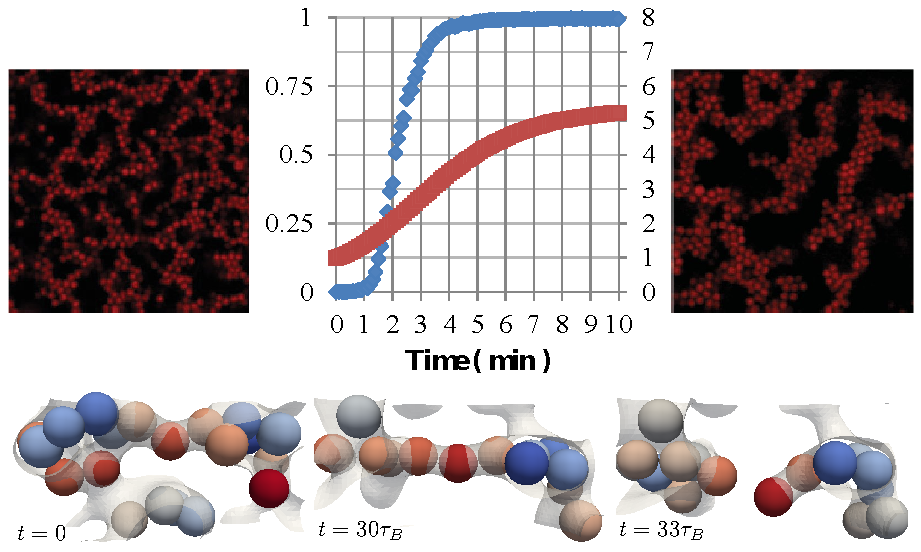
\includegraphics{generate-figure2.pdf}
	\end{center}
	\caption{\textbf{Gelation in dense samples.} \textbf{a} Typical time evolution of the largest cluster size and of the mean coordination number. Insets: Confocal images (2D) at percolation and at final stage. \textbf{b-d} Typical arm-breaking event, from relaxed, to stretched, to rupture. Particles are drawn to scale and colors indicate potential energies from blue (low) to red (high). The smooth surface is a Gaussian coarse-graining of the network pattern. %\textbf{e-f} Typical loop compaction event.  \textbf{b-f} are top views, thus there is no direct role of sedimentation.
	}
	\label{fig:dense}
\end{figure}

\clearpage
\begin{figure}
	\begin{center}
	%\includegraphics{generate-figure3.pdf}
	\end{center}
	\caption{\textbf{Percolation vs compaction} for the three systems studied here: fluid (not percolating), dilute gel and dense gel.}
	\label{fig:general}
\end{figure}
\end{document}